% ============================================================================
% reSTITCHing: journal extension of STITCH (MLCAD '26), v10 (Overleaf build)
% ----------------------------------------------------------------------------
% Self-contained: compiles with pdflatex alone ("latexmk -pdf main.tex", or one
% click on Overleaf), with figures/ next to this file. ASCII only, no em-dashes.
% Supplementary material: supplement.tex ("Supplementary Material Sn").
%
% Generated content (do not edit by hand):
%   the NUMBERS block below <- python -B phase2/frontier/make_numbers_set4.py
%   figures/fig_floor_heatmap.pdf <- the same script
%   every other figures/*.pdf <- python -B paper/make_v10_figures.py
%
% Projections: Claude Haiku 4.5 is incomplete on the RTLLM floor tier. Values
% projected for its missing cells are typeset with \proj{} (italic, dagger).
% \finaltrue makes any remaining projection a compile error.
% ============================================================================
\documentclass[11pt]{article}

\usepackage[margin=1in]{geometry}
\usepackage[T1]{fontenc}
\usepackage{amsmath}
\usepackage{newtxtext,newtxmath}
\usepackage[varqu,varl,scaled=0.95]{zi4}
\usepackage{microtype}
\usepackage{graphicx}
\usepackage{xcolor}
\usepackage{booktabs,tabularx,makecell}
\usepackage{siunitx}
\usepackage{caption}
\usepackage{subcaption}
\usepackage{enumitem}
\usepackage{tikz}
\usetikzlibrary{arrows.meta,positioning,calc,fit}
\usepackage[section]{placeins}
\usepackage{titlesec}
\usepackage{hyperref}
\usepackage[capitalise,noabbrev,nameinlink]{cleveref}

\hypersetup{colorlinks=true, linkcolor=blue!45!black, urlcolor=blue!45!black, citecolor=blue!45!black,
  pdftitle={reSTITCHing: Replicated, Cost-Controlled, and Sign-off-Aware Repair of LLM-Generated RTL}}
\graphicspath{{figures/}}

% ---- layout: floats stay near their first mention ---------------------------
\renewcommand{\topfraction}{0.9}
\renewcommand{\bottomfraction}{0.8}
\renewcommand{\textfraction}{0.07}
\renewcommand{\floatpagefraction}{0.8}
\setcounter{topnumber}{3}
\setcounter{bottomnumber}{2}
\setcounter{totalnumber}{4}
\setlength{\textfloatsep}{10pt plus 3pt minus 2pt}
\setlength{\floatsep}{8pt plus 2pt minus 2pt}
\setlength{\intextsep}{8pt plus 2pt minus 2pt}
\setlength{\emergencystretch}{1.5em}
\captionsetup{font=small, labelfont=bf, labelsep=period, skip=4pt}
\captionsetup[table]{position=top}
\captionsetup[sub]{font=small, labelfont=bf, skip=2pt}
\titleformat{\section}{\large\bfseries}{\thesection}{0.6em}{}
\titleformat{\subsection}{\normalsize\bfseries}{\thesubsection}{0.6em}{}
\titlespacing*{\section}{0pt}{1.5ex plus 0.5ex minus 0.3ex}{0.7ex plus 0.2ex}
\titlespacing*{\subsection}{0pt}{1.2ex plus 0.4ex minus 0.2ex}{0.5ex plus 0.2ex}
\setlist{itemsep=0.1em, topsep=0.25em, leftmargin=1.2em}
\sisetup{group-separator={,}, group-minimum-digits=4, retain-explicit-plus=true}
\crefname{subfigure}{Figure}{Figures}

% ---- colours shared with paper/figstyle.py (one per condition) --------------
\definecolor{cBase}{HTML}{8F8E89}
\definecolor{cGate}{HTML}{E3A835}
\definecolor{cRaw}{HTML}{D9622B}
\definecolor{cVtwo}{HTML}{6FA8E6}
\definecolor{cVthree}{HTML}{1D5AA6}
\definecolor{cEsc}{HTML}{006E4B}

\newcommand{\Supp}[1]{Supplementary Material~S#1}
\newcommand{\cond}[1]{\texttt{#1}}

% ---- projected values (Haiku, RTLLM floor tier) -----------------------------
\newif\iffinal
\finalfalse   % \finaltrue for the submission: any projection left is an error
\newcommand{\projcheck}{\iffinal\errmessage{Projected Haiku values remain}\fi}
\newcommand{\proj}[1]{\projcheck\textit{#1}\textsuperscript{\dag}}

% BEGIN GENERATED NUMBERS
% GENERATED by phase2/frontier/make_numbers_set4.py -- do not edit by hand.
\newcommand{\SetFourRuns}{612}  % set4_analysis.json runs_total
\newcommand{\SetFourErrored}{0}  % set4_analysis.json runs_errored
\newcommand{\SetFourPooledBase}{99.3}  % pass_rates pooled|baseline
\newcommand{\SetFourPooledBaseK}{152/153}  % pass_rates pooled|baseline
\newcommand{\SetFourPooledAdv}{98.7}  % pass_rates pooled|sem_adv
\newcommand{\SetFourPooledAdvK}{151/153}  % pass_rates pooled|sem_adv
\newcommand{\SetFourPooledEsc}{98.0}  % pass_rates pooled|sem_escalate
\newcommand{\SetFourPooledEscK}{150/153}  % pass_rates pooled|sem_escalate
\newcommand{\SetFourPooledRestart}{98.0}  % pass_rates pooled|sem_escalate_restart
\newcommand{\SetFourPooledRestartK}{150/153}  % pass_rates pooled|sem_escalate_restart
\newcommand{\SetFourGPTBaseK}{50/51}  % pass_rates gpt-4.1-mini-2025-04-14|baseline
\newcommand{\SetFourGPTToolRed}{70.5}  % tools gpt-4.1-mini-2025-04-14 reduction_pct
\newcommand{\SetFourGeminiBaseK}{51/51}  % pass_rates gemini-2.5-flash|baseline
\newcommand{\SetFourGeminiToolRed}{100.0}  % tools gemini-2.5-flash reduction_pct
\newcommand{\SetFourHaikuBaseK}{51/51}  % pass_rates claude-haiku-4-5-20251001|baseline
\newcommand{\SetFourHaikuToolRed}{96.5}  % tools claude-haiku-4-5-20251001 reduction_pct
\newcommand{\SetFourGPTDeltaAdv}{$-$2.0}  % contrasts gpt-4.1-mini-2025-04-14|sem_adv
\newcommand{\SetFourGPTDeltaEsc}{$-$3.9}  % contrasts gpt-4.1-mini-2025-04-14|sem_escalate
\newcommand{\SetFourGPTDeltaRestart}{$-$3.9}  % contrasts gpt-4.1-mini-2025-04-14|sem_escalate_restart
\newcommand{\SetFourMinP}{1.000}  % contrasts, min sign-flip p over all scopes and conditions
\newcommand{\SetFourToolRed}{88.6}  % tools pooled reduction_pct
\newcommand{\SetFourToolAdv}{2.29}  % tools pooled sem_adv
\newcommand{\SetFourToolEsc}{0.26}  % tools pooled sem_escalate
\newcommand{\SetFourInrPassMin}{0.11}  % cost, min inr_per_pass over model x condition
\newcommand{\SetFourInrPassMax}{0.51}  % cost, max inr_per_pass over model x condition
\newcommand{\SetFourFingerprintMain}{256}  % fingerprint_counts fp_b43877da5b
\newcommand{\SetFourFingerprintOther}{7}  % fingerprint_counts fp_6050bec882
\newcommand{\SetFourParitySim}{140/140}  % parity_check_osscad.json a_agree/candidates
\newcommand{\SetFourParityInterp}{51/51}  % parity_check_osscad.json b_agree/b_checked
\newcommand{\SetFourBPlanned}{228}  % 19 modules x 4 conditions x N=3
\newcommand{\SetFourBGPTValid}{228}  % set4b_analysis.json coverage gpt-4.1-mini-2025-04-14 valid
\newcommand{\SetFourBGPTErrored}{0}  % coverage gpt-4.1-mini-2025-04-14 errored
\newcommand{\SetFourBGeminiValid}{228}  % set4b_analysis.json coverage gemini-2.5-flash valid
\newcommand{\SetFourBGeminiErrored}{0}  % coverage gemini-2.5-flash errored
\newcommand{\SetFourBHaikuValid}{143}  % set4b_analysis.json coverage claude-haiku-4-5-20251001 valid
\newcommand{\SetFourBHaikuErrored}{85}  % coverage claude-haiku-4-5-20251001 errored
\newcommand{\SetFourBHaikuPending}{85}  % planned - Haiku valid
\newcommand{\SetFourBValidTotal}{599}  % coverage, sum of valid runs
\newcommand{\SetFourAllValid}{1{,}211}  % Set 4 valid runs + Set 4b valid runs
\newcommand{\SetFourBFloorModules}{19}  % Q1 modules
\newcommand{\SetFourBLeaveFloor}{16}  % Q1: modules with a non-floor baseline tier for at least one model
\newcommand{\SetFourBCeilingAll}{4}  % Q1: modules at ceiling for all three models (all three measured)
\newcommand{\SetFourBStillFloor}{\texttt{adder\_pipe\_64bit}, \texttt{alu} and \texttt{freq\_divbyfrac}}  % Q1: floor for every model that ran them
\newcommand{\SetFourBToolFails}{188}  % Q2: fails in the three tool conditions
\newcommand{\SetFourBToolFailsSF}{103}  % Q2: of those, with semantic_fired
\newcommand{\SetFourBToolFailsSFPct}{55}  % Q2: percentage
\newcommand{\SetFourBDBPZeroCells}{3}  % Q2: passes with a directive before the pass in baseline-0/3 cells (all traced, none attributable)
\newcommand{\SetFourBMinP}{0.062}  % Q3: min sign-flip p
\newcommand{\SetFourBQThreeContrasts}{12}  % Q3: number of contrasts
\newcommand{\SetFourBAllThreeModules}{12}  % Q4: modules every model ran
\newcommand{\SetFourBQFour}{\texttt{freq\_divbyfrac}}  % Q4 strict list
\newcommand{\SetFourBQFourRuns}{36}  % Q4: valid runs on the strict module
\newcommand{\SetFourBAluGemini}{3/12}  % Q4_table alu gemini
\newcommand{\SetFourBHaikuModules}{12}  % Q1: modules with Haiku baseline runs
\newcommand{\SetFourBProjCells}{29}  % set4b_haiku_projection.json projected_cells
\newcommand{\SetFourBProjOffset}{+0.72}  % set4b_haiku_projection.json offset_logit
\newcommand{\SetFourBProjOffsetCells}{47}  % set4b_haiku_projection.json offset_cells
\newcommand{\SetFourBCeilingAllClause}{, and \proj{8} of all 19 once Haiku's missing modules are projected}  % Q1 ceiling for all three over all modules, Haiku projected where not run
\newcommand{\SetFourBProjNote}{Haiku: 12 of 19 modules measured; values marked~\textsuperscript{\dag} (hatched in the heat map) are projections, to be replaced.\projcheck{}}  % empty once no projected cell remains
% END GENERATED NUMBERS

\title{\textbf{reSTITCHing: Replicated, Cost-Controlled, and Sign-off-Aware\\Repair of LLM-Generated RTL}}
\author{Karthikeya Patana \and Yashwant Rajesh \and Aathira Sunil \and Durga Saranyu \and Sri Parameswaran \and Kamesh Chandrasekar \and Paresh Saxena \and Soumya Joshi}
\date{}

\begin{document}
\maketitle

% ============================================================================
\begin{abstract}
\noindent STITCH (MLCAD~'26) adds a deterministic interpreter to a language-model
repair loop for Verilog: it translates Verilator lint and Yosys synthesis output
into targeted repair directives. Its evidence was single-run illustrations. This
extension replicates every claim at $N{=}3$ and asks when the interpreter
helps, at what cost, and whether it matters on real hardware.
On RTLLM~v2.1 ($42$ modules, six open models from $4$B to $32$B and three
non-reasoning API models), two interpreter illustrations replicate; firing the
interpreter on every iteration trails baseline by about four points on small
models (not significant); and conditional escalation with a restart matches
baseline on small models ($0.0$ points, cell-level $95\%$ CI $-4.6$ to $+4.6$)
while its cut in heavyweight tool calls grows from $16.6\%$ to $27.6\%$ to
$88.6\%$ up the capability ladder. On an independently developed RISC-V MPSoC
with a mesh network-on-chip ($1{,}386$ runs, seven models), scored by a
specification-complete sign-off testbench, simulation-only repair signs off
$63\%$ of its runs defective, including every simulation-silent defect at every
model size. On the latch-bearing tasks, latch-free clean synthesis rises from
$24\%$ to $88\%$ with the interpreter, a count from Yosys alone. A
pre-registered control arm shows that the detail, not the alarm, drives repair:
the alarm that sign-off failed is worth no more than raw tool text, while
escalation adds $19.7$ points over it (CI $+11.1$ to $+29.3$), and
interpretation beats raw text by $14.1$ points with $23\%$ fewer model calls.
Repaired leaf modules restore synthesis of $4$- and $9$-router meshes, which
simulation-only repair never does.
\end{abstract}

% ============================================================================
\section{Introduction}
\label{sec:intro}

A language model that writes Verilog can be put in a loop: generate, simulate,
feed the simulator's verdict back, and retry, as AutoChip
does~\cite{autochip}. A simulator, however, is blind to a class of defects that
decide whether a design can be signed off: inferred latches, multi-driven nets,
and resets a synthesis tool cannot map all simulate correctly on the inputs a
testbench drives. STITCH~\cite{stitch26} adds Verilator~\cite{verilator} and
Yosys~\cite{yosys} to the loop and places a deterministic interpreter between
the tools and the model, which turns raw diagnostics into short repair
directives at no inference cost. The conference paper characterised the
interpreter through four outcome regimes (enabling, protective, harmful,
irrelevant), each shown by one module and model evaluated once.

This article asks four questions that single runs cannot answer: \emph{when}
the interpreter helps, \emph{how much}, \emph{at what cost}, and \emph{for
which models}, and then a fifth: whether it matters on a real multiprocessor
design. \Cref{fig:teaser} previews the answer to the fifth: on real MPSoC
leaves, a simulation-only loop signs off defective RTL, while the lint and
synthesis layer removes the latches and lets the full designs synthesise.

\begin{figure}[!t]
\centering
\begin{subfigure}[t]{2.08in}
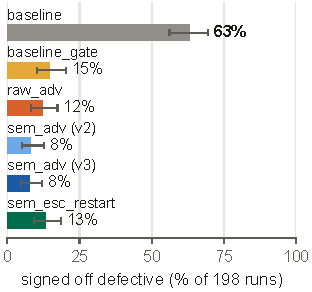
\includegraphics{fig_teaser_a}
\caption{Signed off defective}
\label{fig:teaser-a}
\end{subfigure}\hfill
\begin{subfigure}[t]{2.08in}
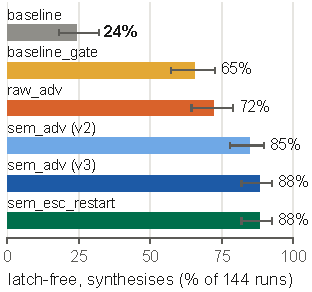
\includegraphics{fig_teaser_b}
\caption{Latch-bearing tasks}
\label{fig:teaser-b}
\end{subfigure}\hfill
\begin{subfigure}[t]{2.08in}
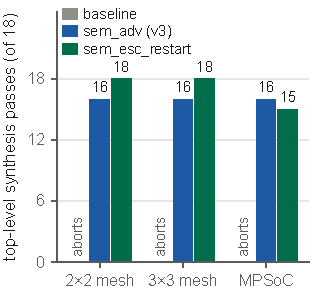
\includegraphics{fig_teaser_c}
\caption{Top-level synthesis restored}
\label{fig:teaser-c}
\end{subfigure}
\caption{STITCH on a real RISC-V MPSoC (six models, $198$ runs per condition).
(a)~A simulation-only loop signs off $63\%$ of its runs as defective; with the
lint and synthesis layer it is $8$ to $15\%$. (b)~On the eight latch-bearing
tasks, runs that end latch-free with a clean synthesis rise from $24\%$ to
$88\%$. (c)~Splicing each condition's repaired leaves back into the $4$- and
$9$-router meshes and the MPSoC top: simulation-only repair never yields a
design that synthesises; v3 and escalation do in $15$ to $18$ of $18$ (model,
replicate) groups. Wilson $95\%$ CI.}
\label{fig:teaser}
\end{figure}

One discipline runs throughout: no interpreter claim is made without
$N{\geq}3$ replication and a check that the interpreter actually fired
(\cond{semantic\_fired}) in the runs it is credited with. The contributions are:
\begin{itemize}
\item \textbf{Replication.} Two interpreter illustrations replicate $3/3$; an
input/output reachability asymmetry explains which defect classes the
interpreter can reach; three larger candidates are retired
(\cref{sec:replication}).
\item \textbf{Cost-controlled escalation} that behaves as baseline until a run
is demonstrably stuck, with its guarantee stated at its true scope; its cut in
heavyweight tool calls grows with model capability (\cref{sec:escalation,sec:rtllm}).
\item \textbf{Harness hardening.} Three silent harness defects, one of which
misclassified $31\%$ of runs, and a structural pass-detection interface
(\cref{sec:harness}).
\item \textbf{RTLLM at scale.} $2{,}124$ replicated STITCH runs on six open
models, a fine-tuning twin comparison with a negative result, and
$\SetFourAllValid$ runs on three commercial non-reasoning API models, including
the floor tier (\cref{sec:design,sec:rtllm}).
\item \textbf{A real-MPSoC case study} with a specification-complete sign-off
oracle, a pre-registered control arm that separates the alarm from the detail,
and an additive interpreter upgrade. Latch-free clean synthesis on the
latch-bearing tasks rises from $24\%$ to $88\%$, and repaired leaves restore
synthesis of $4$- and $9$-router meshes (\cref{sec:mpsoc}).
\end{itemize}

\textbf{Relation to the conference version.} The conference
paper~\cite{stitch26} introduced STITCH: the Verilator and Yosys layer, the
interpreter, a $20$-module in-house suite, and the four outcome regimes, each
illustrated by a single run. \Cref{sec:stitch} recaps that design.
Everything else is new: the $N{=}3$ replication and the retirements, the
escalation policies, the harness corrections, the RTLLM study (Sets~1 to~4),
the fine-tuning twin, the MPSoC case study with the v3 interpreter layer, the
sign-off oracle and the control arm. Two conference readings are revised: the
harmful regime survives only as a non-significant deficit on small models, and
the irrelevant regime (failures with no tool-visible signal) gains a measured
counterpart, the RTLLM floor tier, which turns out to be mostly beyond small open
models rather than beyond the tools.

% ============================================================================
\section{Related Work}
\label{sec:related}

\textbf{Benchmarks and fine-tuned generators.} VerilogEval~\cite{verilogeval}
and RTLLM~\cite{lu2024rtllm} score generated RTL against reference testbenches;
we use RTLLM~v2.1. RTLCoder~\cite{rtlcoder} fine-tunes a code model on curated
Verilog; because it shares base weights with
DeepSeek-Coder~\cite{deepseekcoder}, it allows the twin comparison of
\cref{sec:design}.

\textbf{Feedback loops.} Self-Refine~\cite{selfrefine} established iterative
refinement with self-generated feedback. AutoChip~\cite{autochip} feeds
compilation errors and simulation mismatches back to the model, and
RTLFixer~\cite{rtlfixer} repairs RTL syntax errors from compiler feedback.
Qiu et al.~\cite{qiu2024} use language models to explain EDA tool errors to
learners. STITCH sits in this line but changes what is fed back: synthesis and
lint diagnostics, translated deterministically, with no extra model call.

\textbf{Agentic systems.} Recent systems orchestrate several agents and tools.
VerilogCoder~\cite{verilogcoder} combines a task planner with a syntax checker,
a simulator and an AST-based waveform tracer; MAGE~\cite{mage} samples
high-temperature candidates and debugs them with a Verilog-state checkpoint
mechanism; AIvril~\cite{aivril} runs a multi-agent loop of syntax correction and
functional verification; MEIC~\cite{meic} iterates language-model debugging over
syntax and functional errors; and UVLLM~\cite{uvllm} couples language models
with UVM-based testing and repair. These systems add model calls or agents to
reach higher pass rates. Our contribution is orthogonal: a zero-inference-cost
translation layer, evaluated with replication, per-tier decomposition, a
sign-off oracle that the repair loop never sees, and a control arm that
separates being told \emph{that} a check failed from being told \emph{what}
failed.

% ============================================================================
\section{STITCH in Brief}
\label{sec:stitch}

\Cref{fig:pipeline} shows the loop. Each iteration, the model returns RTL
for a specification; Icarus Verilog~\cite{iverilog} simulates it against a
loop testbench; on failure the loop feeds back the simulation log and,
depending on the condition, the Verilator and Yosys output, raw or interpreted.
The interpreter (\cref{tab:rules}) maps each recognised diagnostic to a
directive that names the signal and the fix; it is a fixed set of rules and
calls no model.

\begin{figure}[!htbp]
\centering
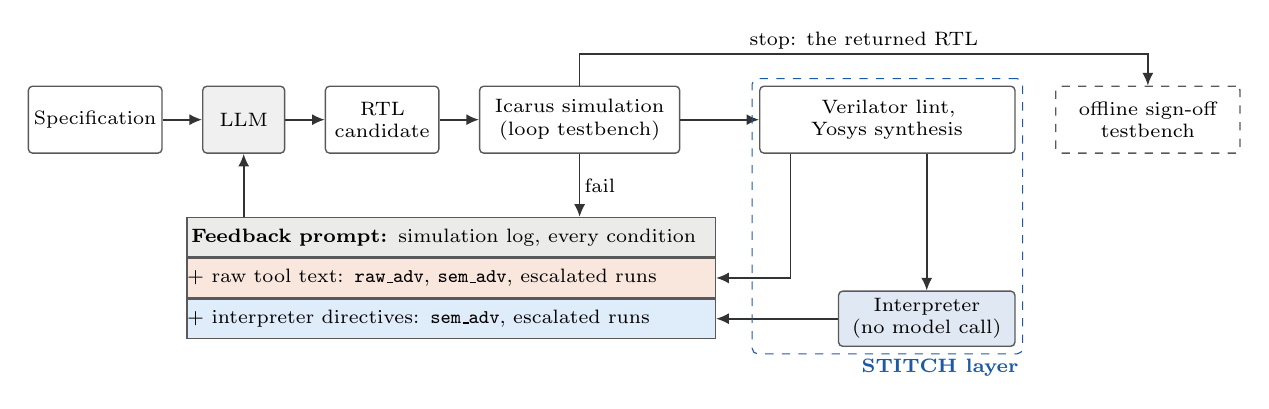
\begin{tikzpicture}[font=\scriptsize, >={Latex[length=1.6mm,width=1.4mm]},
  box/.style={draw=black!65, rounded corners=1.5pt, align=center, minimum height=8.5mm, inner sep=2pt, line width=0.5pt},
  part/.style={draw=black!65, align=left, text width=66mm, minimum height=5mm, inner sep=1.6pt, font=\scriptsize, line width=0.5pt},
  arr/.style={->, line width=0.6pt, draw=black!80},
  lab/.style={font=\scriptsize, inner sep=1.5pt}]
% row 1: generate, simulate, run the tools; sign-off scoring sits outside the loop
\node[box] (spec) {Specification};
\node[box, text width=9mm, fill=black!6, right=5mm of spec] (llm) {LLM};
\node[box, text width=13mm, right=5mm of llm] (rtl) {RTL\\candidate};
\node[box, text width=24mm, right=5mm of rtl] (sim) {Icarus simulation\\(loop testbench)};
\node[box, text width=31mm, right=10mm of sim] (tools) {Verilator lint,\\Yosys synthesis};
\node[box, dashed, text width=22mm, right=5mm of tools] (sign) {offline sign-off\\testbench};
% row 2: the feedback prompt, one line per source, and the interpreter
\node[part, fill=cBase!18, anchor=north west] (f1) at ($(llm.south west)+(-2mm,-8mm)$) {\textbf{Feedback prompt:} simulation log, every condition};
\node[part, fill=cRaw!16, below=0pt of f1] (f2) {+ raw tool text: \cond{raw\_adv}, \cond{sem\_adv}, escalated runs};
\node[part, fill=cVtwo!22, below=0pt of f2] (f3) {+ interpreter directives: \cond{sem\_adv}, escalated runs};
\node[box, text width=21mm, minimum height=7mm, fill=cVthree!14, anchor=east] (interp) at (tools.east |- f3) {Interpreter\\(no model call)};
% arrows: anchor to anchor, orthogonal
\draw[arr] (spec) -- (llm);
\draw[arr] (llm) -- (rtl);
\draw[arr] (rtl) -- (sim);
\draw[arr] (sim) -- (tools);
\draw[arr] (sim.south) -- node[right, lab]{fail} (sim.south |- f1.north);
\draw[arr] ($(tools.south west)+(4mm,0)$) |- (f2.east);
\draw[arr] (interp.north |- tools.south) -- (interp.north);
\draw[arr] (interp.west) -- (f3.east);
\draw[arr] (llm.south |- f1.north) -- (llm.south);
\draw[arr] (sim.north) -- ++(0,4mm) -| node[pos=0.25, above, lab]{stop: the returned RTL} (sign.north);
\node[draw=cVthree, dashed, rounded corners=2pt, inner sep=2.5pt, fit=(tools)(interp)] (stitch) {};
\node[font=\scriptsize\bfseries, text=cVthree, anchor=north east, inner sep=1.5pt] at (stitch.south east) {STITCH layer};
\end{tikzpicture}
\caption{The STITCH loop. \cond{baseline} feeds back the simulation log only;
\cond{raw\_adv} adds the raw tool text; \cond{sem\_adv} adds the interpreter's
directives on every iteration; the escalation policies (\cref{fig:esc}) add
them only once a run is stuck. The Phase~3 sign-off testbench scores the
returned RTL and never reaches the loop.}
\label{fig:pipeline}
\end{figure}

\begin{table}[!htbp]
\centering
\footnotesize
\caption{Interpreter rule classes. v2 is the production interpreter used in
every phase; v3 is the additive layer of \cref{sec:mpsoc}, which reproduces v2
byte for byte wherever no new rule applies. Verification status per class:
\Supp{1}.}
\label{tab:rules}
\begin{tabularx}{\linewidth}{@{}l l X@{}}
\toprule
Class & Source & Directive, in short \\
\midrule
\multicolumn{3}{@{}l}{\emph{v2 (production)}} \\
\cond{UNUSEDSIGNAL} & Verilator & a declared input is never read: use it (e.g.\ gate the output on it) \\
\cond{MULTIDRIVEN} & Verilator & a signal has several drivers: keep one \\
\cond{UNDRIVEN} & Verilator & an output is never assigned, or a name is undeclared \\
\cond{WIDTHTRUNC/EXPAND} & Verilator & a width mismatch on an assignment: size the operands \\
\cond{BLKSEQ}, \cond{COMBDLY} & Verilator & blocking or delayed assignment in the wrong block type \\
Latch inferred & Yosys & assign every output on every path of the block \\
Combinational loop & Yosys & break the feedback path \\
\addlinespace
\multicolumn{3}{@{}l}{\emph{v3 additions}} \\
\cond{MISSING\_CLOCK} & fusion & Yosys latch in a level-sensitive block plus Verilator unused clock: make it edge-triggered \\
\cond{ASYNC\_RESET} & Yosys & ``multiple edge sensitive events'' abort: one asynchronous reset, other clears synchronous \\
\cond{WIDTH\_EXPR} & Verilator & width warning on an expression, which v2 dropped \\
\cond{COMB\_LOOP} & Verilator & \cond{UNOPTFLAT} when Yosys reports no loop \\
\bottomrule
\end{tabularx}
\end{table}

% ============================================================================
\section{Replicated Cases, and What Replication Retired}
\label{sec:replication}

The conference paper's cleanest illustration, a gated input that the model
declares but never reads, replicates $3/3$ on two modules and two models
(\cref{tab:proven}). Verilator fires \cond{UNUSEDSIGNAL}, the directive
names the gating port, and gemma3:4b passes in two iterations where both
controls fail all six. \cond{raw\_adv} tracks \cond{baseline} exactly, so the
effect is the interpretation, not the presence of the tools. The two survivors
are deliberately the same mechanism: other candidates built to elicit it were
discarded because the specification gave the answer away, or because the
system prompt already forced the missing default.

\begin{table}[!htbp]
\centering
\footnotesize
\caption{The two replicated illustrations, $N{=}3$, $T{=}0.1$: outcome and
iterations, identical in all three replicates. Only the interpreter turns
gemma3:4b's failures into passes.}
\label{tab:proven}
\begin{tabular}{@{}l l c c c@{}}
\toprule
Module & Model & \cond{baseline} & \cond{raw\_adv} & \cond{sem\_adv} \\
\midrule
\texttt{decoder\_3to8} & gemma3:4b & FAIL, 6 & FAIL, 6 & \textbf{PASS, 2} \\
\texttt{decoder\_3to8} & llama3.1  & PASS, 2 & PASS, 2 & PASS, 2 \\
\texttt{mux4\_oe}      & gemma3:4b & FAIL, 6 & FAIL, 6 & \textbf{PASS, 2} \\
\texttt{mux4\_oe}      & llama3.1  & PASS, 4 & PASS, 4 & PASS, 2 \\
\bottomrule
\end{tabular}
\end{table}

\textbf{A reachability asymmetry.} A forgotten gating \emph{input} reliably
produces the target defect, but a forgotten \emph{output} does not: on the two
diagnostic modules built for it (\texttt{adder\_with\_overflow},
\texttt{fsm\_next\_state\_error}) gemma3:4b assigned every declared output
unprompted on iteration one, so the interpreter correctly had nothing to fire on
(\cond{semantic\_fired}${=}0$). Driving a declared output is a local obligation
that a model closes by itself; reading a declared input is a non-local one, and
a module that ignores an input still compiles and looks complete.
Reachability is therefore a joint property of the tool and of the generator's
failure distribution, and it has to be measured per class.

\textbf{What replication retired.} Three larger candidates were built to test
whether the mechanism scales, and none survived. On
\texttt{datapath\_mux\_alu}, llama3.1 passed \cond{sem\_adv} in $2$ of $3$
replicates with \cond{semantic\_fired}${=}0$ in all three: a single run would
have read as a win, and it was sampling variance. On
\texttt{instr\_decode\_unit}, gemma3:4b received the correct directive and still
failed, falling into a syntax loop the interpreter has no vocabulary for; and
\texttt{alu\_with\_enable} became too easy after its redesign. The in-house
benchmark showed the same fragility at scale: re-measured at $N{=}3$, $4$ of its
$5$ ``real-test'' cells and $2$ of its $3$ ``enabling'' cells did not reproduce
the baseline behaviour their category was defined by (\Supp{2}).

% ============================================================================
\section{Cost-Controlled Escalation}
\label{sec:escalation}

Firing the interpreter on every iteration intervenes when no intervention is
needed and can derail a run that was converging. The escalation policies
(\cref{fig:esc}) intervene only once a run is stuck. Each iteration generates
RTL and simulates it, and a pass stops the run in any state. A failure yields a
normalised error signature (the first $5$ lines of the log). In the
\emph{baseline} state only the simulation log is fed back; after $N{=}2$
consecutive failures with the same signature the run switches permanently to the
\emph{escalated} state from the next iteration, which feeds back the simulation
log, the tool text and the directives, as \cond{sem\_adv} does. The restart
variant, after $M{=}3$ further same-signature failures, issues one blank-slate
prompt that discards the current RTL and stays escalated. The budget is eight
iterations on RTLLM.

\begin{figure}[!htbp]
\centering
\begin{minipage}[t]{0.52\linewidth}
\centering
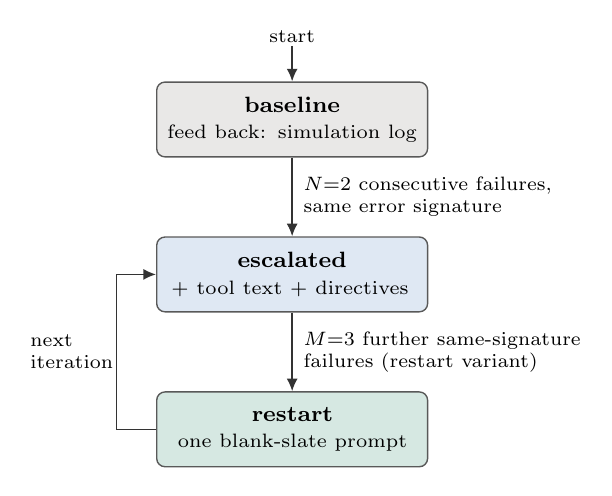
\begin{tikzpicture}[baseline=(current bounding box.north), font=\footnotesize, >={Latex[length=1.6mm,width=1.4mm]},
  st/.style={draw=black!65, rounded corners=3pt, align=center, text width=33mm, minimum height=9.5mm, inner sep=2pt, line width=0.5pt},
  arr/.style={->, line width=0.6pt, draw=black!80},
  lab/.style={font=\scriptsize, align=left, inner sep=1pt}]
\node[st, fill=cBase!20] (b) {\textbf{baseline}\\{\scriptsize feed back: simulation log}};
\node[st, fill=cVthree!14, below=10mm of b] (e) {\textbf{escalated}\\{\scriptsize + tool text + directives}};
\node[st, fill=cEsc!16, below=10mm of e] (r) {\textbf{restart}\\{\scriptsize one blank-slate prompt}};
\draw[arr] ($(b.north)+(0,4.5mm)$) node[above, lab]{start} -- (b.north);
\draw[arr] (b.south) -- node[right, lab, xshift=1mm]{$N{=}2$ consecutive failures,\\same error signature} (e.north);
\draw[arr] (e.south) -- node[right, lab, xshift=1mm]{$M{=}3$ further same-signature\\failures (restart variant)} (r.north);
\draw[arr] (r.west) -- ++(-5mm,0) |- node[pos=0.25, left, lab]{next\\iteration} (e.west);
\end{tikzpicture}
\captionof{figure}{Escalation state machine. A pass stops the run in any
state; until the first trigger, an escalation run is a \cond{baseline} run.}
\label{fig:esc}
\end{minipage}\hfill
\begin{minipage}[t]{0.44\linewidth}
\centering
\footnotesize
\captionof{table}{Cost per run, all $255$ in-house benchmark runs: escalation
calls the heavyweight tools least.}
\label{tab:cost}
\begin{tabular}{@{}l r r@{}}
\toprule
Condition & \makecell[r]{Tokens\\per run} & \makecell[r]{Tool calls\\per run} \\
\midrule
\cond{baseline}        & 4,891 & 0.00 \\
\cond{raw\_adv}        & 5,354 & 2.61 \\
\cond{sem\_adv}        & 4,883 & 2.37 \\
\cond{sem\_escalate}   & 5,151 & \textbf{1.53} \\
\cond{sem\_esc\_restart} & 4,719 & \textbf{1.37} \\
\bottomrule
\end{tabular}
\end{minipage}
\end{figure}

Until the trigger, an escalation run receives exactly the prompts and feedback
a \cond{baseline} run receives, so \emph{on runs that converge before the
trigger it is the baseline policy}. Beyond the trigger it diverges, and nothing
guarantees that it does as well as baseline from there: it may help or hurt. A
worst case equal to baseline can therefore be claimed only for the runs that
converge before the trigger. Whether the divergence costs anything is an
empirical question. On the Set~1 recoverable band (\cref{sec:rtllm}),
\cond{sem\_escalate\_restart} matches baseline ($0.0$ points, cell-level $95\%$
CI $-4.6$ to $+4.6$, $p{=}1.000$), while plain \cond{sem\_escalate} trails it
like always-on interpretation ($-4.7$, CI $-10.7$ to $0.0$, $p{=}0.148$, against
$-4.6$, CI $-10.5$ to $+0.7$, for \cond{sem\_adv}).

On the $255$-run in-house benchmark, escalation invokes the heavyweight tools
(Verilator and Yosys) $35$ to $45\%$ less often than always-on interpretation
and raw tool text at a matching or better pass rate (\cref{tab:cost}). The two
cost axes differ: escalated runs execute extra iterations, so tokens can rise
while tool calls fall. Every efficiency claim below is scoped to the tool-call
axis.

% ============================================================================
\section{Harness Hardening}
\label{sec:harness}

We found and fixed three silent defects in the shared runner, each verified
against golden references before and after. (A) The simulator ran without a
working directory, so a testbench that loads a data file with
\texttt{\$readmemh} could never pass. (B) An unclosed code fence left the
opening marker in the extracted code, corrupting $58$ of $659$ generated files
($8.8\%$). (C) The pass check looked for \texttt{"PASS"}, while RTLLM
testbenches print \texttt{"Your Design Passed"}: a re-scan found $20$ of $64$
completed runs ($31\%$) misclassified as failures, which then spent their
remaining iterations ``fixing'' correct code. All three are one fragility: an
assumption about a benchmark's output format, buried in shared code, that
produces plausible wrong numbers. Every confirmatory result here therefore
routes pass detection through one function, \texttt{detect\_outcome(log,
benchmark)}, backed by a per-benchmark registry with no default, so an
unregistered benchmark fails at import rather than silently (\Supp{3}).

% ============================================================================
\section{RTLLM Study Design and the Fine-Tuning Twin}
\label{sec:design}

\textbf{Pool and tiers.} A compatibility screen of RTLLM~v2.1~\cite{lu2024rtllm}
kept $44$ of $50$ designs (one exclusion is a defect in RTLLM's own reference);
two more were dropped because their testbenches pass stuck-at-$0$ outputs,
leaving $42$ modules. A pilot showed that STITCH's effect is visible only where
baseline sometimes fails but can recover, so modules are tiered by the maximum
baseline pass rate across the five Twin model-conditions: \emph{ceiling}
($6$ modules, ${\geq}80\%$), \emph{recoverable} ($17$, $20$ to $80\%$) and
\emph{floor} ($19$, ${<}20\%$).

\textbf{Runs.} All use the hardened harness, $N{=}3$ and local Ollama
serving~\cite{ollama} for open models:
\begin{itemize}
\item Set~2 (Twin): $5$ model-conditions $\times 42$ modules, $630$ runs,
\cond{baseline} only, $T{=}0.5$.
\item Set~1: gemma3:4b~\cite{gemma3}, llama3.1:8b~\cite{llama3},
deepseek-coder:6.7b, four conditions, $42$ modules: $1{,}512$ runs, $T{=}0.1$.
\item Set~3: qwen2.5-coder:14b and 32b~\cite{qwen25coder} and gemma3:27b, four
conditions, the $17$ recoverable modules: $612$ runs, $T{=}0.1$.
\item Sets~4 and 4b: three API models, recoverable band ($\SetFourRuns$ runs)
and floor ($\SetFourBValidTotal$ valid runs), $T{=}0.1$ (\cref{sec:api}).
\end{itemize}
\cond{baseline} and \cond{sem\_adv} are capped at six iterations and the
escalation policies at eight; at an equal cap of six no Set~1 or Set~3
conclusion changes. Sets~1 and~3 had $6$ and $2$ timeouts, excluded and counted
(\Supp{5}).

\textbf{The fine-tuning twin.} RTLCoder-Deepseek-v1.1~\cite{rtlcoder,rtlcoder_hf}
is fine-tuned from the same weights as deepseek-coder:6.7b, so the pair
isolates fine-tuning. On the recoverable band, at the shared prompt, RTLCoder
passes $21/51$ against the base model's $32/51$: $0$ module wins, $13$ ties
($|\Delta|\leq1$ of $3$) and $4$ losses. At RTLCoder's native prompt it is a
wash ($29/51$; $5$ wins, $6$ ties, $6$ losses). The four losses trace to a
submodule-hierarchy mismatch, dialect leakage, a parameter-binding failure and a
memorised folder name used as the module name. Fine-tuning does help on one
class: RTLCoder (native) clears every recoverable signal-processing module
($9/9$) and the recoverable memory module ($3/3$). Prompt format alone has a
modest, inconsistent effect (native $3$ wins, shared $2$, $12$ ties). So on this
external benchmark fine-tuning shows no net advantage, a negative result with a
per-class exception (\Supp{4}).

% ============================================================================
\section{STITCH at RTLLM Scale}
\label{sec:rtllm}

\subsection{Small models (Set 1): where always-on interpretation stands}
\label{sec:set1}

Pooled over all $42$ modules the four conditions lie within $1.6$ points
($28.8$, $27.2$, $27.7$ and $28.8\%$); pooling ceilings with floors hides any
signal. Split by tier (\cref{fig:set1}), three findings appear.
\textbf{(1)} On the recoverable band, \cond{sem\_adv} is about four points
below baseline ($47/153$ against $54/153$): worse in $7$ of $51$ (module, model)
cells, better in $3$, equal in $41$, cell-level $95\%$ CI $-10.5$ to $+0.7$,
sign-flip $p{=}0.199$. The direction is the conference paper's harmful regime,
but the deficit is not distinguishable from zero, it is not uniform across
models, and Set~1 has no \cond{raw\_adv} condition, so it cannot be separated
from the effect of the raw tool text that accompanies the directives.
\textbf{(2)} \cond{sem\_escalate\_restart} matches baseline ($54/151$ against
$54/153$; $0.0$, CI $-4.6$ to $+4.6$), and plain \cond{sem\_escalate} does not
($47/150$; $-4.7$, CI $-10.7$ to $0.0$). \textbf{(3)} On ceilings and floors
all conditions coincide ($80$ to $85\%$ and $6$ to $7\%$).

\begin{figure}[!htbp]
\centering
\begin{subfigure}[t]{3.15in}
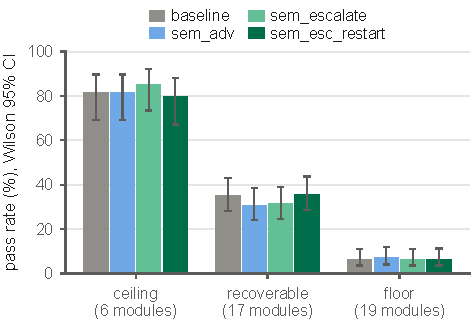
\includegraphics{fig_set1_tiers}
\caption{Pass rate by tier and condition}
\label{fig:set1-a}
\end{subfigure}\hfill
\begin{subfigure}[t]{3.15in}
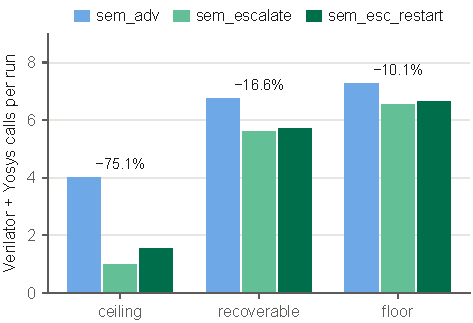
\includegraphics{fig_set1_calls}
\caption{Verilator and Yosys calls per run}
\label{fig:set1-b}
\end{subfigure}
\caption{Set~1, three models from $4$B to $8$B, $1{,}512$ runs. (a)~The
conditions differ only on the recoverable band, and there within noise.
(b)~Escalation's cut in tool calls against always-on interpretation follows the
tier: $75.1\%$ on ceilings, $16.6\%$ on the recoverable band, $10.1\%$ on floors
($18.5\%$ pooled).}
\label{fig:set1}
\end{figure}

\textbf{Cost.} Where baseline succeeds, the two-strike trigger almost never
fires, and escalation cuts tool calls from $4.02$ to $1.00$ per run on ceilings;
where runs get stuck it does fire, and the cut is $16.6\%$ on the recoverable
band and $10.1\%$ on floors (\cref{fig:set1-b}). Tokens move the other way,
as on the in-house benchmark.

\subsection{Up the ladder (Set 3): the deficit fades, the cost advantage grows}
\label{sec:set3}

On three larger models ($14$B to $32$B), the mean \cond{sem\_adv} minus
baseline difference shrinks from $-4.6$ points to $-0.65$, and no contrast
differs from baseline: \cond{sem\_adv} $-0.7$ (CI $-7.8$ to $+6.5$),
\cond{sem\_escalate} $+2.6$ (CI $-1.3$ to $+7.2$), \cond{sem\_escalate\_restart}
$+2.0$ (CI $-2.6$ to $+7.2$), all $p\geq0.40$. The nominal escalation lead
($90/153$ against $86/153$) is not a fired mechanism: of $153$
\cond{sem\_escalate} runs, $88$ passed without escalating, $65$ escalated, and
the $2$ of those that passed did so with \cond{semantic\_fired}${=}0$, rescued by
raw tool feedback. Per model the deficit is not monotonic in size
(\cref{fig:ladder-b}): gemma3:27b reverses it ($+7.8$) while
qwen2.5-coder:32b keeps it ($-5.9$), every interval crossing zero. The cost
advantage, a mechanical count, does grow: on the recoverable band escalation
cuts tool calls by $27.6\%$ ($5.31$ to $3.85$ per run) against $16.6\%$ for the
small models, because capable models get stuck less often.

\begin{figure}[!htbp]
\centering
\begin{subfigure}[t]{3.15in}
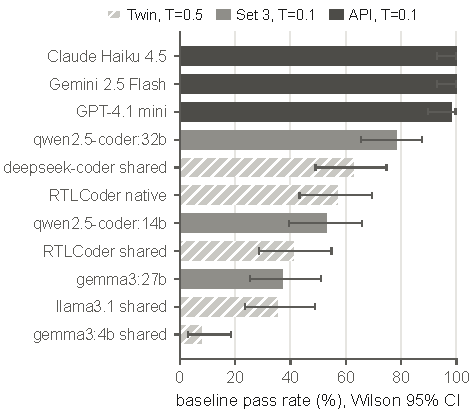
\includegraphics{fig_ladder}
\caption{Baseline pass rate, every model}
\label{fig:ladder-a}
\end{subfigure}\hfill
\begin{subfigure}[t]{3.15in}
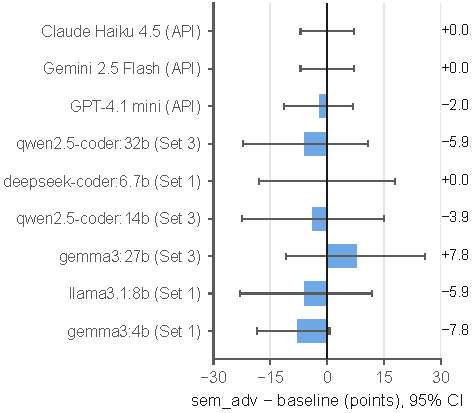
\includegraphics{fig_deficit}
\caption{Always-on interpretation minus baseline}
\label{fig:ladder-b}
\end{subfigure}
\caption{The capability ladder on the $17$ recoverable modules. (a)~Baseline
pass rate for every model in the study, with Wilson intervals~\cite{wilson1927};
the Twin bars ran at $T{=}0.5$, so the ladder is ordinal across shades. (b)~The
always-on deficit, with Newcombe $95\%$ intervals for a difference of two
proportions~\cite{newcombe1998}, ordered by baseline pass rate: it is small,
not monotonic in model size, and every interval crosses zero.}
\label{fig:ladder}
\end{figure}

\subsection{Commercial non-reasoning API models (Sets 4 and 4b)}
\label{sec:api}

Set~4 runs the Set~3 protocol unchanged on \texttt{gpt-4.1-mini-2025-04-14},
\texttt{gemini-2.5-flash} (thinking budget $0$) and
\texttt{claude-haiku-4-5-20251001}: $T{=}0.1$, no reasoning tokens (checked on
every call), and a laptop toolchain matched to the cluster build (Yosys~$0.69$,
Verilator~$5.053$, Icarus~$14.0$), whose verdicts reproduce saved Set~3
candidates exactly ($\SetFourParitySim$ pass/fail, $\SetFourParityInterp$
interpreter outputs). It was pre-registered, with each amendment hashed before
the calls it governs.

\textbf{Recoverable band: a ceiling.} Pooled pass rates are $\SetFourPooledBase$,
$\SetFourPooledAdv$, $\SetFourPooledEsc$ and $\SetFourPooledRestart\%$ for the
four conditions. Gemini and Haiku pass every run, so the condition comparison
rests on GPT-4.1 mini alone, where the three tool conditions differ from
baseline by \SetFourGPTDeltaAdv, \SetFourGPTDeltaEsc{} and
\SetFourGPTDeltaRestart{} points, all on one module, with no significant
contrast (every sign-flip $p{=}\SetFourMinP$). Escalation rarely triggers, so
its tool-call cut reaches $\SetFourToolRed\%$ ($\SetFourToolAdv$ to
$\SetFourToolEsc$ calls per run; $\SetFourGPTToolRed$ to
$\SetFourGeminiToolRed\%$ per model): the trend runs
$16.6\%\rightarrow27.6\%\rightarrow\SetFourToolRed\%$ up the ladder. Each
passing module cost INR~$\SetFourInrPassMin$ to $\SetFourInrPassMax$.

\textbf{Floor (Set 4b).} On the $\SetFourBFloorModules$ floor modules
(\cref{fig:floor}), $\SetFourBLeaveFloor$ leave the floor at baseline for at
least one API model, so the floor is mostly a property of the $4$B to $32$B
models, not of the modules. $\SetFourBCeilingAll$ of the
$\SetFourBAllThreeModules$ modules all three models ran are at ceiling for all
three\SetFourBCeilingAllClause. \SetFourBProjNote{}
\SetFourBStillFloor{} stay at the floor for every model that ran them. On the
remaining failures the interpreter does fire, in
$\SetFourBToolFailsSFPct\%$ ($\SetFourBToolFailsSF/\SetFourBToolFails$) of the
failing tool-condition runs, but no pass is attributable to it. Only
$\SetFourBDBPZeroCells$ passes followed a directive in a cell whose baseline was
$0/3$; in one of the two cells the same gain appears in runs that received no
directive, and in the other the directive was followed by several compile-error
iterations before the pass. No condition contrast is significant (smallest
$p{=}\SetFourBMinP$ of $\SetFourBQThreeContrasts$). Of the
$\SetFourBAllThreeModules$ modules every model ran, only \SetFourBQFour{} fails
in all $\SetFourBQFourRuns$ runs; we analyse it in \cref{sec:floorcase}.

\begin{figure}[!htbp]
\centering
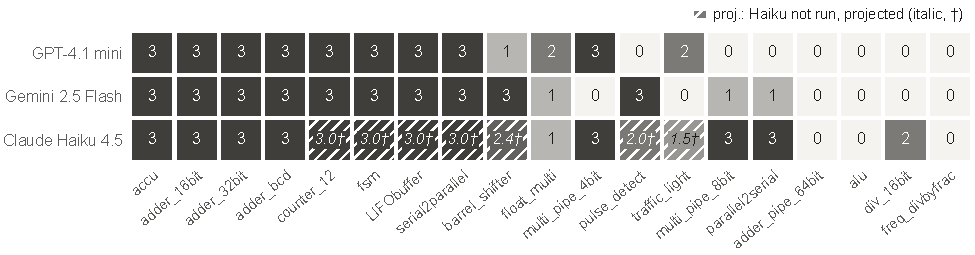
\includegraphics{fig_floor_heatmap}
\caption{Set~4b, the $\SetFourBFloorModules$ RTLLM floor modules: baseline
passes of $3$ per module and API model, ordered by the GPT-4.1 mini and
Gemini~2.5 Flash passes. Most modules the open models could not pass are passed
by at least one API model; three stay at the floor for every model.
\SetFourBProjNote}
\label{fig:floor}
\end{figure}

\textbf{Disclosures.} Claude Haiku~4.5 is incomplete on the floor tier
($\SetFourBHaikuValid/\SetFourBPlanned$ runs; $\SetFourBHaikuPending$ failed on
exhausted account credit and are excluded), so every observed floor result rests
on the runs each model completed, and the fails-everywhere test on the modules
all three models ran. A fourth model (Kimi) was dropped at its smoke test.
OpenAI's serving fingerprint changed during the run ($\SetFourFingerprintMain$
and $\SetFourFingerprintOther$ calls) for the same pinned snapshot. RTLLM has
been public since 2024, so training contamination may inflate absolute pass
rates; it does not affect the within-model contrasts. Details: \Supp{6}.

\subsection{freq\_divbyfrac: a specification-wording defect, not a testbench defect}
\label{sec:floorcase}

All three API models fail \texttt{freq\_divbyfrac} ($0/36$), a $3.5\times$
clock divider whose specification says that the output stays high for $3$ half
clock steps and low for $4$. Its reference design passes its testbench, and the
testbench's expected waveform matches that sentence. Running every final
candidate through the original testbench, none is a phase-shifted copy of the
expected waveform (the reference itself fails when shifted by one step); all
$34$ that compile have the wrong period and duty cycle, typically high for $6$
to $7$ and low for $7$ half steps, and $32$ fail first at check~3. Simulating
the reference with its counter exposed shows why the specification misleads:
the counter advances once per rising edge, so it wraps every $14$ half steps
and the reference emits two output periods per wrap, while the specification
states that ``the counter cycles through $7$ half clock steps''. So this is not
a testbench defect; the specification's own description of the counter does not
match its reference design (our reading), and the models fail on period and
duty cycle, roughly doubling the period. The testbench also releases reset in
the same time step as a clock edge, a minor robustness weakness that did not
cause these failures, since no candidate fails by a phase offset (\Supp{7}).

\subsection{What the RTLLM study establishes}
\label{sec:rtllm-summary}

\begin{enumerate}
\item The illustration mechanism generalises to a per-tier prediction: the
interpreter acts where it can reach a real defect and stays silent elsewhere.
\item Always-on interpretation trails baseline by about four points on the
small models' recoverable band, consistent in direction (worse in $7$ of $51$
cells, better in $3$) but not significant at $N{=}3$, and not separable from
the raw tool text it accompanies.
\item Escalation is the baseline policy on every run that converges before its
trigger; beyond the trigger only its restart variant matches baseline on small
models ($0.0$, CI $-4.6$ to $+4.6$), while plain escalation trails like always-on
interpretation ($-4.7$, CI $-10.7$ to $0.0$). On large and API models every
condition matches baseline within noise.
\item The deficit is a small-model phenomenon at the group level, non-monotonic
per model; there is no large-model pass-rate win for escalation.
\item The tool-call cut is tier-shaped and grows with capability: $16.6\%$,
$27.6\%$ and $\SetFourToolRed\%$ on the recoverable band.
\item The floor is mostly beyond small open models, not beyond the tools; where
API models still fail, the interpreter fires but no pass is attributable to it.
\end{enumerate}
RTLLM scores a module by its testbench alone, and on the recoverable band the
interpreter had something to say in only about a third of always-on runs ($52$
of $153$ in Set~1). It cannot measure what STITCH was built for: defects that
pass the testbench, break synthesis, and multiply when a module is instantiated
across a real design.

% ============================================================================
\section{An MPSoC Case Study}
\label{sec:mpsoc}

\subsection{Substrate: real RTL that already contains the target defects}
\label{sec:mpsoc-substrate}

The design is an in-group MPSoC: a five-stage RV32 core, a network interface,
and a virtual-channel wormhole mesh router, built as a $2{\times}2$ and a
$3{\times}3$ mesh. Only compile-level changes were made for the open-source
flow. Synthesis of the MPSoC top reports $63$ latch inferences across $12$
module definitions and then aborts: a one-bit register tests
\texttt{clr | reset} inside an asynchronous-reset block, which Yosys cannot map.
These defects are \emph{simulation-silent}: the latching multiplexers behave
correctly on their intended inputs, and the aborting register simulates
correctly. Both meshes inherit two latching register definitions, each
instantiated $20$ times per router: Yosys prints one message per definition, so
the feedback is the same at $4$ and $9$ routers while the damage scales with
router count, $2{,}880$ latch cells in the $2{\times}2$ mesh and $6{,}480$ in the
$3{\times}3$ ($9/4$ of it; abort-causing file excluded; \cref{fig:compose-a}).
With the task leaves repaired, both meshes synthesise with $0$ latch cells and
the MPSoC top with $122$, left in five modules outside the repair set, so its
bound is restored synthesis rather than a latch-free design (\Supp{8}). Because
the top-level testbench is a weak oracle, top-level claims are structural;
functional claims rest on per-module testbenches.

\begin{figure}[!htbp]
\centering
\begin{subfigure}[t]{3.15in}
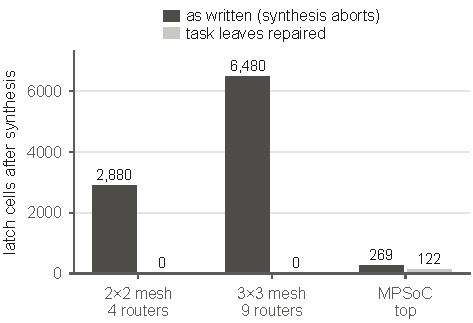
\includegraphics{fig_latch_scale}
\caption{The latch defect at scale}
\label{fig:compose-a}
\end{subfigure}\hfill
\begin{subfigure}[t]{3.15in}
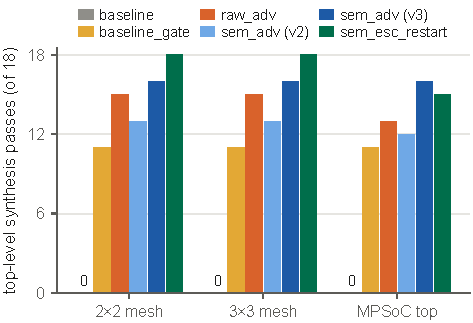
\includegraphics{fig_compose}
\caption{Top-level synthesis after repair, by condition}
\label{fig:compose-b}
\end{subfigure}
\caption{Leaf defects in the real designs. (a)~Two latching register
definitions, instantiated in every router, give latch cells in proportion to
the router count, while Yosys prints the same two messages; with the task
leaves repaired, both meshes have none. (b)~Splicing each condition's repaired
leaves back in ($18$ model and replicate groups per design): simulation-only
repair never restores synthesis, because it never touches the sim-silent
register that aborts it.}
\label{fig:compose}
\end{figure}

\textbf{Keeping the interpreter robust.} Running the production interpreter
(v2) on the real logs exposed gaps synthetic tests had not: an unused clock got
the generic gating template (\texttt{if (clk)} in a combinational block, which
builds a clock-gated latch); the asynchronous-reset abort and a truncation
whose operand is an expression produced no directive. The v3 layer
(\cref{tab:rules}) imports v2 unchanged, reproduces it byte for byte
wherever no new rule applies, and adds rules only where a real log showed the
production directive wrong or missing; its key rule fuses a Yosys latch with a
Verilator unused-clock warning into a missing-clock-edge diagnosis. A live drift
gate caught a latch-message format change between Yosys~$0.33$ and $0.69$ that
would otherwise have silently disabled the new rules (\Supp{8}).

\subsection{Experiment}
\label{sec:mpsoc-exp}

\textbf{Tasks.} Eleven repair tasks (\cref{tab:tasks}): the eight
defective real leaves and three seeded modules for classes absent from the
reference. Six are simulation-silent: the defective input already passes its
loop testbench. Specifications are purely behavioural; a pilot with hint-bearing
specifications let an $8$B model fix every defect on its first call under every
condition, so the hints were removed.

\begin{table}[!htbp]
\centering
\footnotesize
\caption{The eleven repair tasks. Src: R, a real MPSoC leaf; S, seeded for a
class absent from the design. Sim-silent: the defective input already passes
its loop testbench. Sign-off TB: whether the sign-off testbench differs from
the loop testbench.}
\label{tab:tasks}
\begin{tabular}{@{}l c l l c@{}}
\toprule
Task & Src & Defect (v3 class) & Stratum & Sign-off TB \\
\midrule
\texttt{MuxPC}, \texttt{execute\_mux}, \texttt{mux3} & R & latch (\cond{LATCH}) & sim-silent & same \\
\texttt{mem\_wb\_mux}     & R & latch (\cond{LATCH}) & sim-silent & differs \\
\texttt{register\_1bit}   & R & unmappable async reset (\cond{ASYNC\_RESET}) & sim-silent & same \\
\texttt{riscv\_alu\_flags} & S & latch on ALU flags (\cond{LATCH}) & sim-silent & same \\
\texttt{Address\_select}  & R & latch, width-mismatched port & sim-visible & differs \\
\texttt{register\_32bit}, \texttt{register\_4bit} & R & missing clock edge (\cond{MISSING\_CLOCK}) & sim-visible & same \\
\texttt{noc\_xbar4}       & S & multi-driven output (\cond{MULTIDRIVEN}) & sim-visible & same \\
\texttt{ni\_flit\_pack}   & S & width truncation (\cond{WIDTH\_EXPR}) & sim-visible & same \\
\bottomrule
\end{tabular}
\end{table}

\textbf{Conditions.} All share one budget of six model calls, the same prompt,
and identically filtered raw tool text, and every candidate is fully evaluated;
the conditions differ only in what is fed back. Each run starts from the
defective input, evaluated before the first call. \cond{baseline} stops at the
first simulation pass, as AutoChip does, so on a sim-silent task it stops at the
input. \cond{raw\_adv} adds raw Verilator and Yosys lines; \cond{sem\_adv} adds
v2 or v3 directives; \cond{sem\_esc\_restart} (v3) starts like baseline behind a
generic message (``the design simulates correctly but fails synthesis
sign-off''), escalates to v3 after two identical signatures and restarts once.
The control arm \cond{baseline\_gate} gives simulation feedback plus exactly that
message, stops at a clean pass and never escalates; the v3 interpretation of each
RTL it sees is logged, never fed back.

\textbf{Models and pre-registration.} Six local models from $3$B to $14$B
(llama3.2:3b, gemma3:4b, deepseek-coder:6.7b, qwen2.5-coder:7b, llama3.1:8b,
qwen2.5-coder:14b), $N{=}3$, $T{=}0.1$, ran the first five conditions on the
institutional GPU cluster ($990$ runs). The control arm (same six models,
$198$ runs) and qwen2.5-coder:32b (all six conditions, $198$ runs) were
pre-registered before any of their runs, with four primary contrasts and their
readings, frozen with the runner, interpreter and task files: $1{,}386$ cluster
runs in all. Three API models (GPT-4.1 mini, Claude Haiku~4.5, Gemini~2.5 Flash,
$198$ runs each) ran the same runner code, prompts and toolchain as descriptive
ladder rows.

\textbf{Two oracles.} Each task has a \emph{loop testbench}, which drives
feedback and stopping, and a \emph{specification-complete sign-off testbench},
which scores the returned RTL offline and never reaches the loop. The sign-off
testbench was added after a formal-equivalence audit (Result~8) found two
testbench gaps; on the other nine tasks the two testbenches are identical.
Re-scoring the $990$ runs is exact, post hoc for those runs and pre-registered
for the new arms. A run is \emph{sign-off clean} (the primary metric) when the
sign-off testbench passes \emph{and} Yosys reports no latch or loop \emph{and}
Verilator no hard structural warning; it is \emph{signed off defective} when the
loop testbench passed it but it is not sign-off clean; \emph{loop-clean} is the
same structural rule under the loop testbench, the first write-up's metric, kept
as a sensitivity. The three replicates of a (model, task) cell are correlated,
so contrasts use a bootstrap interval and a sign-flip test over the $66$ cells,
about $1.7$ times wider than a per-run Wilson interval.

\subsection{Results}
\label{sec:mpsoc-results}

\textbf{(1) Latches: on the latch-bearing tasks, runs that end latch-free with
a clean synthesis rise from 24\% under simulation-only repair to 88\% under v3
and escalation} ($35/144$ against $127/144$; \cref{fig:teaser-b}), against
$85\%$ ($122/144$) with v2, $72\%$ ($104/144$) with raw text and $65\%$
($94/144$) with the alarm alone. This count uses Yosys only, so it depends on
neither testbench. Simulation-only repair signs off defective RTL at every size:
\cond{baseline} passes its loop testbench in $85\%$ of runs but is sign-off
clean in $22\%$, and $125$ of its $198$ runs ($63\%$) are signed off defective
(\cref{tab:mpsoc-cond}, \cref{fig:teaser-a}), including all $108$ sim-silent
runs, where it stops before any model call. The same holds up the ladder: all
$18$ sim-silent runs are signed off defective for qwen2.5-coder:32b and for each
API model. With the lint and synthesis layer, signed-off-defective runs fall to
$8\%$ (v2, v3), $12\%$ (raw text) and $13\%$ (escalation).

\begin{table}[!htbp]
\centering
\footnotesize
\caption{Phase~3 by condition, six models, $198$ runs each. Escalation is
sign-off clean most often; with any tool feedback, signed off defective falls
from $63\%$ to $8$ to $15\%$. Sign-off clean with Wilson $95\%$ CI.}
\label{tab:mpsoc-cond}
\begin{tabular}{@{}l rcr rr rr@{}}
\toprule
 & \multicolumn{3}{c}{Sign-off} & \multicolumn{2}{c}{Loop} & \multicolumn{2}{c}{Cost} \\
\cmidrule(lr){2-4}\cmidrule(lr){5-6}\cmidrule(l){7-8}
Condition & \makecell[r]{clean\\\%} & \makecell{95\%\\CI} & \makecell[r]{defective\\\%} & \makecell[r]{pass\\\%} &
  \makecell[r]{clean\\\%} & \makecell[r]{calls\\per run} & \makecell[r]{tokens\\per run} \\
\midrule
\cond{baseline}               & 22 & 17--28 & 63 & 85 & 23 & 1.34 & 1,425 \\
\cond{baseline\_gate}         & 52 & 45--59 & 15 & 67 & 56 & 3.39 & 3,835 \\
\cond{raw\_adv}               & 53 & 46--59 & 12 & 65 & 59 & 3.27 & 4,396 \\
\cond{sem\_adv} (v2)          & 63 & 56--69 & \textbf{8} & 71 & 68 & 2.83 & 3,831 \\
\cond{sem\_adv} (v3)          & 67 & 60--73 & \textbf{8} & 74 & 74 & 2.51 & 3,377 \\
\cond{sem\_esc\_restart} (v3) & \textbf{72} & 65--78 & 13 & 85 & 80 & 2.99 & 3,798 \\
\bottomrule
\end{tabular}
\end{table}

\textbf{(2) What the model is told decides the repair; the alarm alone is not
enough.} Told only that sign-off failed, \cond{baseline\_gate} reaches $52\%$
sign-off clean, level with raw text ($53\%$); interpretation reaches $63\%$ (v2)
and $67\%$ (v3), and escalation $72\%$. In the pre-registered contrasts
(\cref{tab:primary}), contrasts~1 and~2 exclude zero with the alarm lower:
reading R1, \emph{the detail in the feedback adds value beyond the verdict}.
The pre-declared processor-level sensitivity (Result~8) gives the same reading
($+24.2$, CI $+14.6$ to $+34.3$; $+19.7$, CI $+7.6$ to $+32.3$), as does
loop-clean ($+23.7$, $+17.7$). Escalation's advantage holds in both strata;
always-on v3's is carried by the sim-silent tasks (\cref{fig:p3-a}). The alarm
plateaus: from the third call to the sixth it adds two points ($50$ to $52\%$),
while escalation climbs from $56$ to $72\%$ once it hands over to v3
(\cref{fig:p3-b}). The alarm alone breaks working logic: of $108$ sim-silent
alarm-only runs, all starting from RTL that simulates, $80$ still pass the loop
testbench at the end, against $97$ under escalation. And of the $95$ alarm-only
runs that are not sign-off clean, $38$ returned RTL that still carries a defect
v3 names (logged, never fed back). The gain is largest on the smallest models:
escalation over the alarm is $+39.4$ points on llama3.2:3b and $+33.3$ on
gemma3:4b (Holm $p{=}0.006$ each).

\begin{figure}[!htbp]
\centering
\begin{subfigure}[t]{3.15in}
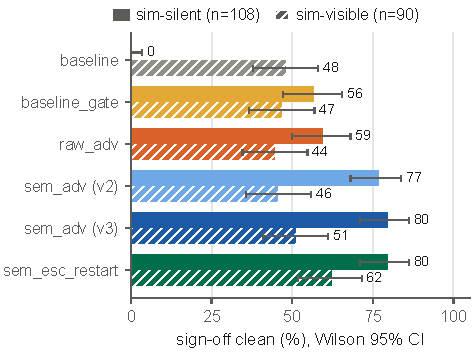
\includegraphics{fig_p3_stratum}
\caption{Sign-off clean by condition and stratum}
\label{fig:p3-a}
\end{subfigure}\hfill
\begin{subfigure}[t]{3.15in}
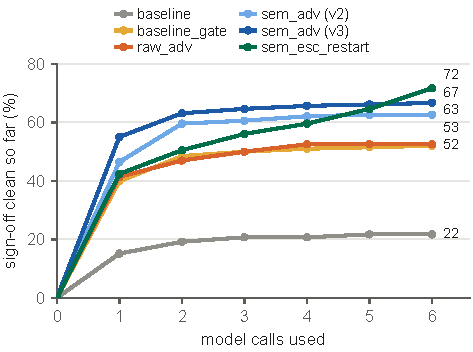
\includegraphics{fig_p3_bycall}
\caption{Sign-off clean after each model call}
\label{fig:p3-b}
\end{subfigure}
\caption{Phase~3, six models. (a)~Simulation-only repair scores $0/108$ on
sim-silent defects by construction; interpretation and escalation lead on them,
and escalation also leads on sim-visible defects. (b)~v3 front-loads its
repairs, the alarm alone plateaus after the third call, and escalation, which
opens with the same alarm, climbs to the highest final rate.}
\label{fig:p3}
\end{figure}

\begin{table}[!htbp]
\centering
\footnotesize
\caption{Pre-registered primary contrasts on sign-off clean, six models:
points, cell-level bootstrap $95\%$ CI, sign-flip $p$, and the runs only A or
only B got right. Escalation and v3 beat the alarm; the alarm is no better than
raw text or simulation alone. Per-stratum rows of contrast~3: \Supp{8}.}
\label{tab:primary}
\begin{tabular}{@{}l l S[table-format=+2.1] S[table-format=+2.1]@{\ to\ }S[table-format=+2.1] r r@{}}
\toprule
Contrast (A $-$ B) & Tasks & {$\Delta$} & \multicolumn{2}{c}{95\% CI} & $p$ & A/B only \\
\midrule
1. \cond{sem\_esc\_restart} $-$ \cond{baseline\_gate} & all & +19.7 & +11.1 & +29.3 & $<$0.001 & 42/3 \\
   & \quad sim-silent  & +23.1 & +11.1 & +37.0 & 0.002 & 27/2 \\
   & \quad sim-visible & +15.6 & +4.4  & +27.8 & 0.022 & 15/1 \\
\addlinespace
2. \cond{sem\_adv} (v3) $-$ \cond{baseline\_gate} & all & +14.6 & +3.0 & +26.3 & 0.021 & 43/14 \\
   & \quad sim-silent  & +23.1 & +6.5  & +39.8 & 0.014 & 31/6 \\
   & \quad sim-visible & +4.4  & -11.1 & +20.0 & 0.688 & 12/8 \\
\addlinespace
3. \cond{baseline\_gate} $-$ \cond{raw\_adv} & all & -0.5 & -9.1 & +8.1 & 1.000 & 16/17 \\
4. \cond{baseline\_gate} $-$ \cond{baseline} & sim-visible & -1.1 & -4.4 & +2.2 & 1.000 & 2/3 \\
\bottomrule
\end{tabular}
\end{table}

\textbf{(3) Interpretation beats raw text, sooner and cheaper.} With the same
raw text and budget, \cond{sem\_adv} (v3) reaches $132/198$ sign-off clean
against \cond{raw\_adv}'s $104/198$: $+14.1$ points (CI $+3.5$ to $+24.7$,
$p{=}0.014$; $40$ discordant pairs against $12$). The production interpreter,
written before this case study and never tuned on its designs, gains $+10.1$
(CI $+2.0$ to $+18.7$, $p{=}0.030$): the out-of-sample estimate of what
interpretation is worth. v3 needs about $23\%$ fewer model calls and tokens per
run, $5{,}066$ against $8{,}370$ tokens per sign-off clean run, and $55\%$ of
its runs are sign-off clean after the first call, against $41\%$ with raw text
and $15\%$ with simulation only. The gain is largest where raw text is hardest
to use: $+24.2$ points on llama3.2:3b and $+27.3$ on qwen2.5-coder:7b; the $14$B
model is at $30/33$ with either.

\textbf{(4) Escalation reaches the highest sign-off clean rate with the fewest
tool rounds.} \cond{sem\_esc\_restart} reaches $72\%$, keeps baseline's $85\%$
loop pass rate, and uses $47.5\%$ fewer tool-feedback rounds than always-on v3.
On the sim-visible tasks, where simulation-only repair does run the model,
escalation beats it by $+14.4$ points ($56/90$ against $43/90$, CI $+3.3$ to
$+27.8$, $p{=}0.048$; $+23.3$ loop-clean, the difference being the
\texttt{Address\_select} gap of Result~8). It protects the smallest model: on
those tasks llama3.2:3b is sign-off clean in $7/15$ runs with simulation only,
$1/15$ with raw text every round, and $8/15$ with escalation.

\textbf{(5) Repaired leaves let the real designs synthesise.} Splicing each
(model, replicate) set of repaired leaves back into the designs
(\cref{fig:compose-b}), simulation-only repair never yields a synthesisable
design, because it never touches the sim-silent register that aborts synthesis;
v3 reaches $16/18$ in each design, escalation $18/18$ in both meshes and
$15/18$ for the MPSoC top, raw text $15$, $15$ and $13$, and the alarm $11/18$
(all conditions: \Supp{8}). In the $990$ runs, loop-clean leaves were
sufficient for composition: whenever all composed leaves were loop-clean, the
design reached its bound ($32/32$, $32/32$, $27/27$).

\textbf{(6) Up the ladder.} \Cref{tab:ladder} adds qwen2.5-coder:32b and
the three API models, one model each at $N{=}3$. At this size any tool feedback
repairs every sim-silent defect ($18/18$ under every tool condition, $16$ or
$18$ under the alarm alone), so interpretation's edge over raw text and over
the alarm vanishes. Every miss outside baseline is on \texttt{Address\_select}
(Result~8), apart from two alarm-only runs on the ALU task for
qwen2.5-coder:32b and for GPT-4.1 mini. Gemini~2.5 Flash's
\texttt{Address\_select} repairs mostly meet the specification ($15/15$
sim-visible under four conditions). Simulation-only repair still signs off all
$18$ sim-silent runs as defective for every model: the interpreter's pass-rate
benefit is a small-model phenomenon, but the guard is needed at every size.

\begin{table}[!htbp]
\centering
\footnotesize
\caption{Ladder rows, one model each, $N{=}3$, descriptive (not pooled with
\cref{tab:mpsoc-cond}): sign-off clean on the sim-silent tasks (sil., of $18$)
and the sim-visible tasks (vis., of $15$), and tokens per run (tok.). Any tool
feedback repairs every sim-silent defect; simulation alone repairs none.}
\label{tab:ladder}
\setlength{\tabcolsep}{3.2pt}
\begin{tabular}{@{}l rrr@{\hspace{11pt}}rrr@{\hspace{11pt}}rrr@{\hspace{11pt}}rrr@{}}
\toprule
 & \multicolumn{3}{c}{Qwen2.5-Coder 32B} & \multicolumn{3}{c}{GPT-4.1 mini} & \multicolumn{3}{c}{Claude Haiku 4.5} & \multicolumn{3}{c}{Gemini 2.5 Flash} \\
\cmidrule(lr){2-4}\cmidrule(lr){5-7}\cmidrule(lr){8-10}\cmidrule(l){11-13}
Condition & sil. & vis. & tok. & sil. & vis. & tok. & sil. & vis. & tok. & sil. & vis. & tok. \\
\midrule
\cond{baseline}               & 0  & 12 & 663   & 0  & 12 & 440   & 0  & 12 & 517   & 0  & 15 & 516 \\
\cond{baseline\_gate}         & 16 & 12 & 1,824 & 16 & 12 & 1,529 & 18 & 12 & 1,099 & 18 & 15 & 1,160 \\
\cond{raw\_adv}               & 18 & 12 & 1,492 & 18 & 12 & 1,164 & 18 & 12 & 1,334 & 18 & 12 & 1,291 \\
\cond{sem\_adv} (v2)          & 18 & 12 & 1,655 & 18 & 12 & 1,255 & 18 & 12 & 1,517 & 18 & 15 & 1,478 \\
\cond{sem\_adv} (v3)          & 18 & 12 & 1,660 & 18 & 12 & 1,257 & 18 & 12 & 1,524 & 18 & 14 & 1,479 \\
\cond{sem\_esc\_restart} (v3) & 18 & 12 & 1,850 & 18 & 12 & 1,404 & 18 & 12 & 1,101 & 18 & 15 & 1,225 \\
\bottomrule
\end{tabular}
\end{table}

\textbf{(7) The upgrade closes the vocabulary gaps.} On the two tasks where v2
produced no directive on the defective input (the async-reset register and the
flit-packing truncation), v3 fires the intended class in $18/18$ runs; on the
two latching registers it replaces the clock-gating directive with the
missing-clock directive; on the address selector it drops a misleading
``gate the output on the instruction bus'' directive. On the async-reset
register, whose abort blocks synthesis of both meshes, interpreter-credited wins
rise from $3/18$ to $15/18$. Across the four tasks singled out before the runs,
sign-off clean rises from $42/72$ to $50/72$ ($+11.1$ points, CI $-9.7$ to
$+31.9$): a favourable direction that remains in-sample, since the v3 rules were
written from these designs' logs.

\textbf{(8) Oracle integrity, and a limitation of structural advice.} The
equivalence audit found two tasks whose loop testbench does not check what the
specification states. In \texttt{mem\_wb\_mux} the conference paper's motivating
case appears in real RTL: a latch holds a stale store operand in exactly the
cases the testbench never drives, and $16$ loop-clean repairs drive an
unspecified value there. In \texttt{Address\_select} the specification defines
\texttt{J\_addr} $= X + \texttt{PC}$ on every input, the testbench checks it
only on a non-flushed jump, and $41$ loop-clean repairs set \texttt{J\_addr} to
$0$ elsewhere: latch-free and synthesisable, yet in violation of the
specification. The production latch directive suggests ``one unconditional
assignment at the top of the block'' of the form \texttt{J\_addr = <safe
value>}. Among the six models' \texttt{Address\_select} runs that are loop-clean
but fail sign-off, that advice appears in all $8$, $12$ and $11$ under v2, v3
and escalation, and in none of the $3$, $7$ and $2$ under simulation only, raw
text and the alarm, which produce such runs without it: a count, not a causal
claim. A structural fix can be functionally wrong exactly where the loop
testbench does not look, and a specification-complete sign-off oracle is what
catches it. At the processor level this violation is invisible (the multiplexer
that consumes \texttt{J\_addr} reads it only on a jump), and the pre-declared
sensitivity that signs \texttt{Address\_select} off with its loop testbench
gives the same reading (Result~2).

\textbf{What the case study establishes.} On real multiprocessor RTL, the
question STITCH answers is whether the design can be signed off, and there a
simulation-only loop is blind at every model size tested. Being told
\emph{that} sign-off failed is worth about as much as raw tool text; being told
\emph{what} failed adds $14.6$ points through interpretation and $19.7$ through
escalation, most on the smallest models, and interpretation does it sooner and
more cheaply than raw text. Leaf repairs compose: fixing a handful of
definitions restores synthesis of networks with $4$ and $9$ routers.

% ============================================================================
\section{Threats to Validity}
\label{sec:threats}

\textbf{Statistical.} Replicates of a cell are correlated, so general claims
rest on cell-level bootstraps; $N{=}3$ leaves the small-model deficit and
several per-model effects undecided. \textbf{Sampling.} One temperature
($T{=}0.1$; Twin $0.5$) and quantised local models served by Ollama; the
control arm ran on a different inference backend (Vulkan rather than CUDA),
with no detectable effect on byte-identical prompts. \textbf{Toolchains.}
Diagnostic formats change between tool versions; a live drift gate caught one
change, and the API runs used a toolchain matched to the cluster build.
\textbf{In-sample interpreter.} The v3 rules were written from the MPSoC logs
and are untested on held-out defects; v2's out-of-sample gain is the
conservative estimate. \textbf{Oracle.} The sign-off testbench is post hoc for
the first $990$ runs (pre-registered for the rest), with loop-clean reported
beside it. \textbf{Benchmark.} RTLLM is public, so API models may have seen it;
this affects absolute rates, not within-model contrasts. \textbf{API coverage.}
Claude Haiku~4.5 is incomplete on the RTLLM floor tier; observed conclusions use
its completed runs only, and the two places that need a complete column mark
projected values. \textbf{API drift.} Hosted models change behind stable names;
snapshots were pinned where possible and returned model versions, fingerprints
and request identifiers were logged for every call. \textbf{Composition} is
checked by synthesis only; composed systems were not simulated.

% ============================================================================
\section{Conclusion and Directions}
\label{sec:conclusion}

STITCH's conference version showed, one run at a time, that an interpreter can
help. On replicated, tier-decomposed evidence the picture is narrower and more
useful. The interpreter acts on the recoverable band, on small models, and only
on defects it can reach; firing it every iteration trails baseline on small
models by a non-significant four points; escalation is the baseline policy until
a run is stuck, matches baseline on small models when it can restart, and cuts
tool calls more the stronger the model ($16.6$, $27.6$ and $\SetFourToolRed\%$).
Non-reasoning API models are at ceiling on the recoverable band and lift
$\SetFourBLeaveFloor$ of the $\SetFourBFloorModules$ floor modules off the floor,
so the floor belongs mostly to small open models; where they still fail, the
interpreter fires but credits no pass. On real hardware, STITCH is best read as
a deterministic sign-off guard and translator: it catches what simulation
misses at every model size, its detail rather than the alarm drives repair, and
the repaired leaves restore synthesis of whole designs, at no inference cost of
its own.

\textbf{Directions.} (i)~Held-out real defects to test the v3 rules out of
sample. (ii)~A latch directive that defaults each signal to the value the
specification defines rather than to a constant, which targets the
\texttt{Address\_select} violations. (iii)~Integration-level feedback for defects
that exist only once modules are connected (a one-bit program-counter port
driven with $32$ bits, a FIFO instantiated positionally with a missing port).
(iv)~Reasoning models, which this study does not cover, and a targeted study of
why the deficit depends on a model's post-training rather than its size.
(v)~Specification-level robustness: in \texttt{freq\_divbyfrac} the
specification's description of the counter does not match its reference design
(our reading) and every model fails, a defect no interpreter can see.

% ============================================================================
\section*{Availability}
Code, runners, analysis scripts, pre-registrations and evidence reports:
\url{https://github.com/Karthik-Flash/STITCH} (an index of the repository is in
\texttt{REPO\_INDEX.md}). Pre-registration hashes (SHA-256): Phase~3 final batch
\texttt{1b6eb915\ldots cc63}; API study \texttt{CC23711D\ldots 653B} (after its
last amendment); API Phase~3 rows \texttt{680F24F5\ldots C130}. The raw result
trees (per-run logs and API ledgers) are not in the repository and are available
on request.

\section*{Acknowledgments}
This work is partially supported by the research project sponsored by
Xilinx-AMD. Opinions and conclusions presented are solely those of the authors
and are not representative of AMD's roadmap. The cluster runs used the
institutional high-performance computing facility of BITS Pilani, Hyderabad
Campus.

% ============================================================================
\begin{thebibliography}{99}
\small
\setlength{\itemsep}{1pt}

\bibitem{stitch26}
K.~Patana, Y.~Rajesh, A.~Sunil, D.~Saranyu, S.~Parameswaran, K.~Chandrasekar,
P.~Saxena, and S.~Joshi, ``STITCH: Semantic Toolchain Integration for
LLM-Driven RTL Circuit and Hardware Design Generation,'' in \emph{Proc. ACM/IEEE
MLCAD}, 2026, doi:10.1145/3831599.3840333.

\bibitem{autochip}
S.~Thakur, J.~Blocklove, H.~Pearce, B.~Tan, S.~Garg, and R.~Karri, ``AutoChip:
Automating HDL Generation Using LLM Feedback,'' arXiv:2311.04887, 2023.

\bibitem{rtlfixer}
Y.~Tsai, M.~Liu, and H.~Ren, ``RTLFixer: Automatically Fixing RTL Syntax Errors
with Large Language Model,'' in \emph{Proc. DAC}, 2024,
doi:10.1145/3649329.3657353.

\bibitem{verilogeval}
M.~Liu, N.~Pinckney, B.~Khailany, and H.~Ren, ``VerilogEval: Evaluating Large
Language Models for Verilog Code Generation,'' in \emph{Proc. ICCAD}, 2023,
doi:10.1109/ICCAD57390.2023.10323812.

\bibitem{lu2024rtllm}
Y.~Lu, S.~Liu, Q.~Zhang, and Z.~Xie, ``RTLLM: An Open-Source Benchmark for
Design RTL Generation with Large Language Model,'' in \emph{Proc. ASP-DAC},
2024, doi:10.1109/ASP-DAC58780.2024.10473904.

\bibitem{rtlcoder}
S.~Liu, W.~Fang, Y.~Lu, Q.~Zhang, H.~Zhang, and Z.~Xie, ``RTLCoder:
Outperforming GPT-3.5 in Design RTL Generation with Our Open-Source Dataset and
Lightweight Solution,'' in \emph{Proc. IEEE LLM Aided Design Workshop (LAD)},
2024, doi:10.1109/LAD62341.2024.10691788.

\bibitem{rtlcoder_hf}
RTLCoder-Deepseek-v1.1, Hugging Face model repository.\newline
\url{https://huggingface.co/ishorn5/RTLCoder-Deepseek-v1.1}

\bibitem{selfrefine}
A.~Madaan et~al., ``Self-Refine: Iterative Refinement with Self-Feedback,'' in
\emph{Advances in Neural Information Processing Systems 36 (NeurIPS)}, 2023.

\bibitem{qiu2024}
S.~Qiu, B.~Tan, and H.~Pearce, ``LLM-aided Explanations of EDA Synthesis
Errors,'' in \emph{Proc. IEEE LLM Aided Design Workshop (LAD)}, 2024,
doi:10.1109/LAD62341.2024.10691721.

\bibitem{verilogcoder}
C.-T.~Ho, H.~Ren, and B.~Khailany, ``VerilogCoder: Autonomous Verilog Coding
Agents with Graph-based Planning and Abstract Syntax Tree (AST)-based Waveform
Tracing Tool,'' in \emph{Proc. AAAI}, 2025, doi:10.1609/aaai.v39i1.32007.

\bibitem{mage}
Y.~Zhao, H.~Zhang, H.~Huang, Z.~Yu, and J.~Zhao, ``MAGE: A Multi-Agent Engine
for Automated RTL Code Generation,'' in \emph{Proc. DAC}, 2025,
doi:10.1109/DAC63849.2025.11133191.

\bibitem{aivril}
M.~ul~Islam, H.~Sami, P.-E.~Gaillardon, and V.~Tenace, ``AIvril: AI-Driven RTL
Generation With Verification In-The-Loop,'' arXiv:2409.11411, 2024.

\bibitem{meic}
K.~Xu et~al., ``MEIC: Re-thinking RTL Debug Automation using LLMs,'' in
\emph{Proc. ICCAD}, 2024, doi:10.1145/3676536.3676801.

\bibitem{uvllm}
Y.~Hu et~al., ``UVLLM: An Automated Universal RTL Verification Framework using
LLMs,'' arXiv:2411.16238, 2024.

\bibitem{deepseekcoder}
D.~Guo et~al., ``DeepSeek-Coder: When the Large Language Model Meets
Programming -- The Rise of Code Intelligence,'' arXiv:2401.14196, 2024.

\bibitem{gemma3}
Gemma Team, ``Gemma 3 Technical Report,'' arXiv:2503.19786, 2025.

\bibitem{llama3}
A.~Grattafiori et~al., ``The Llama 3 Herd of Models,'' arXiv:2407.21783, 2024.

\bibitem{qwen25coder}
B.~Hui et~al., ``Qwen2.5-Coder Technical Report,'' arXiv:2409.12186, 2024.

\bibitem{iverilog}
S.~Williams, ``Icarus Verilog.'' \url{https://steveicarus.github.io/iverilog/}

\bibitem{verilator}
W.~Snyder, ``Verilator.'' \url{https://www.veripool.org/verilator/}

\bibitem{yosys}
C.~Wolf, ``Yosys Open SYnthesis Suite.'' \url{https://yosyshq.net/yosys/}

\bibitem{ollama}
Ollama. \url{https://ollama.com}

\bibitem{wilson1927}
E.~B.~Wilson, ``Probable Inference, the Law of Succession, and Statistical
Inference,'' \emph{J. Amer. Statist. Assoc.}, vol.~22, no.~158, pp.~209--212,
1927, doi:10.1080/01621459.1927.10502953.

\bibitem{newcombe1998}
R.~G.~Newcombe, ``Interval Estimation for the Difference Between Independent
Proportions: Comparison of Eleven Methods,'' \emph{Statistics in Medicine},
vol.~17, no.~8, pp.~873--890, 1998.

\end{thebibliography}

\end{document}
